\chapter{Funcionamento da Aplicação }

A aplicação apresentada tem uma interface muito simples, uma vez que o seu
proprósito é ser utilizado numa linha de comandos.

\section{Menus }
O menu inicial mostra ao utilizador 3 opções: Iniciar sessão, registar na aplicação ou sair. 

\begin{figure}[tbph]
	\centering
	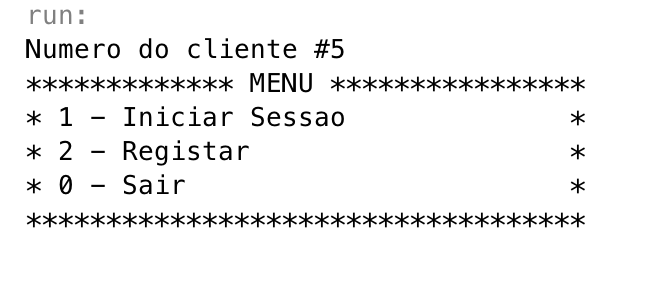
\includegraphics[scale=0.5]{imagem/menuInicial.png}
	\caption{Menu Inicial}
	\label{fig:menuInicial}
\end{figure}

Após o inicio de sessão, o utilizador poderá tentar arranjar equipa ou então efetuar logout. 
\begin{figure}[tbph]
	\centering
	\includegraphics[scale=0.5]{imagem/iniciarSessao.png}
	\caption{Menu de inicio de sessão}
	\label{fig:iniciar sessao}
\end{figure}

Após selecionar a opção entrar numa equipa, o utilizador ficará à espera até ser encontrado uma equipa que tenha outros jogadores com um ranking semelhante ao dele e após ter sido colocado numa equipa é informado que já tem equipa e é mostrada a constituição da equipa dele e a adversária, seguido do menu para escolher o heroi. Quando escolhe o heroi é apresentada uma lista com 30 herois e o utilizador necessita de escolher um. 

\begin{figure}[tbph]
	\centering
	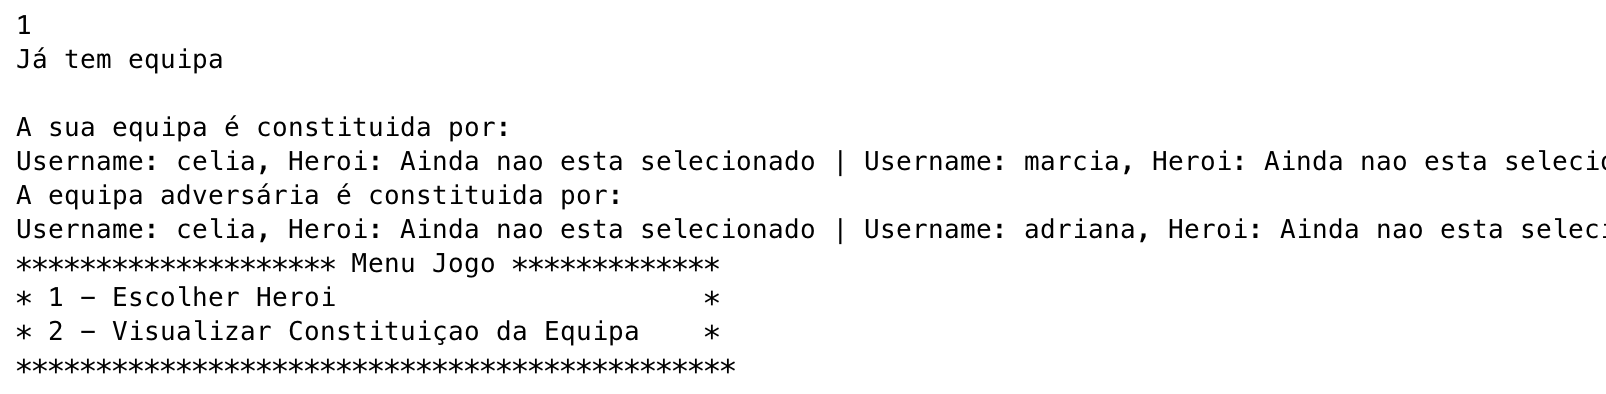
\includegraphics[scale=0.5]{imagem/entrarNumaEquipa.png}
	\caption{Entrar numa equipa}
	\label{fig:Entrarnumaequipa}
\end{figure}

\newpage

Após selecionar o heroi escolhido o utilizador pode confirmar, escolher outro e ainda visualizar a equipa. De notar que o utilizador apenas tem 30 segundos para efetuar a escolha de heroi. 

\begin{figure}[tbph]
	\centering
	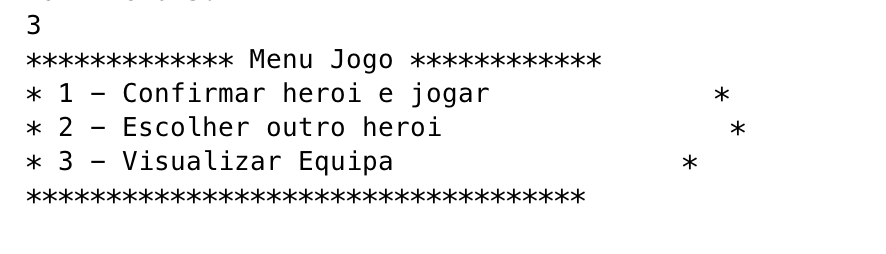
\includegraphics[scale=0.5]{imagem/menuEscolherHeroi.png}
	\caption{Menu para a escolha de heroi}
	\label{fig:escolher heroi}
\end{figure}

Após ser confirmado o herói é gerado um resultado aleatório em que uma das equipas ganha e são atualizados os rakings dos jogadores. Após este acontecimento o jogador poderá tentar jogar outro jogo. 
\begin{figure}[tbph]
	\centering
	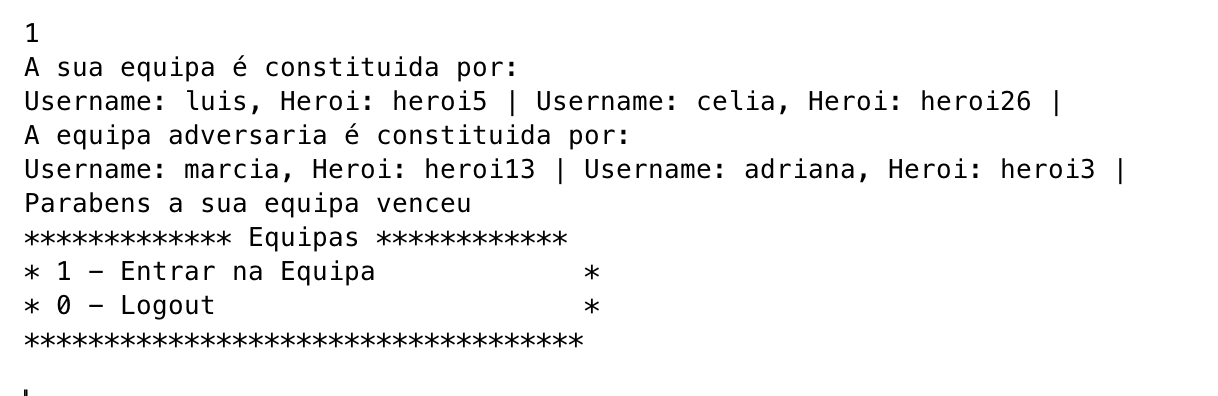
\includegraphics[scale=0.5]{imagem/jogoEfetuado.png}
	\caption{Jogo efetuado com sucesso}
	\label{fig:jogoEfetuado}
\end{figure}




